% \begin{figure}[htbp]
%     \centering
%     \includegraphics[width=0.55\textwidth]
%     {images/newer_phi_plot_N=32 (1).pdf}
%     \caption[An Application of our Adaptive Mesh Refinement Technique to the Two-Dimensional Maxwell Eigenproblem]{The results from applying five iterations of our adaptive mesh refinement technique of Section \ref{AMR} to Algorithm \ref{pseudospec} for the Maxwell operator \eqref{max op}. The blue curve shows $\Phi_h(z, A)$ when no adaptivity is applied. The orange curve shows $\Phi_h(z, A)$ after five iterations of adaptive mesh refinement. The green curve shows the corresponding corrected approximation $\Phi_{h,c}(z, A).$  The black dashed curve shows the exact distance $\operatorname{dist}(z, \Sp{A})$ and the black dots indicate the exact eigenvalues.}
%     \label{DWRResult}
% \end{figure}

% \caption[Application of Adaptive Mesh Refinement to the Two-Dimensional Maxwell Eigenproblem]
% {Results obtained by applying five iterations of the adaptive mesh refinement technique of Section \ref{AMR} to Algorithm \ref{pseudospec} for the Maxwell operator \eqref{max op}. The blue curve shows $\Phi_h(z,A)$ without adaptivity, while the orange curve shows $\Phi_h(z,A)$ after five adaptive refinement iterations. The green curve shows the corresponding corrected approximation $\Phi_{h,c}(z,A)$. The black dashed curve shows the exact distance $\operatorname{dist}(z,\Sp{A})$, and the black dots indicate the exact eigenvalues.}

%%%Bens below


\begin{figure}[htbp]
    \centering
    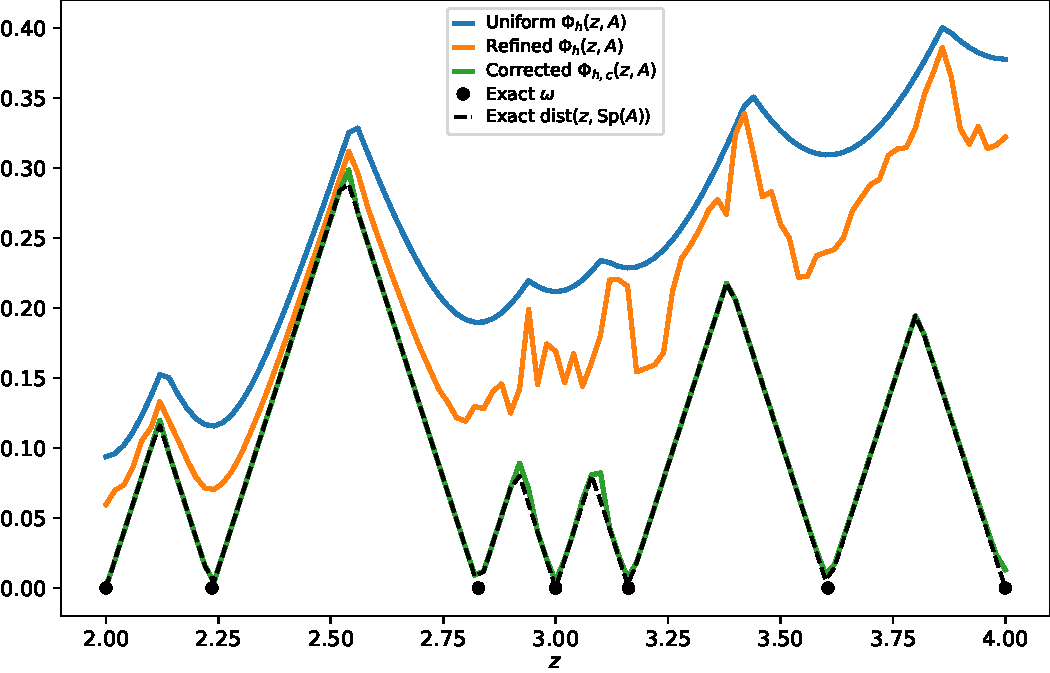
\includegraphics[width=0.55\textwidth]
    {images/cruves.pdf}
    \vspace{-1em}
    \caption[An Application of our Adaptive Mesh Refinement Technique to the Two-Dimensional Maxwell Eigenproblem]{The results from applying five iterations of our adaptive mesh refinement technique of \Cref{AMR} to \Cref{pseudospec} for the Maxwell operator \eqref{max op}. The blue curve shows $\Phi_h(z, A)$ when no adaptivity is applied. The orange curve shows $\Phi_h(z, A)$ after five iterations of adaptive mesh refinement. The green curve shows the corresponding corrected approximation $\Phi_{h,c}(z, A).$  The black dashed curve shows the exact distance $\operatorname{dist}(z, \Sp{A})$ and the black dots indicate the exact eigenvalues. \pef{Does 'uniform' in the caption mean 'before refinement', the same confusion we had in the slides for Matt? If so please change the label and caption, it is confusing.} \pef{This figure is really important and convincing, make it much bigger}}
    \label{DWRResult}
\end{figure}
